\chapter{Simulation}

Statistics attempts to make sense of randomness.  It also uses
randomness in a variety of different ways in computations.  Resampling
methods such as cross-validation take random permutations of the
observations to create test and training sets from the data.
Similarly, the non-parametric bootstrap uses samples from the
observational units, and the parametric bootstrap involves sampling
from probability distributions with parameters that are estimated from
the data.  In simulation studies, also known as Monte Carlo studies,
we apply statistical methods to randomly generated data in order to:
evaluate the effectiveness of a method in a controlled situation,
provide a ``laboratory setting'' for comparing techniques, and give
intuition about the anomalies and variation we see in our data.
Simulation allows us to do ``in silico'' experiments and provides us
with an extraordinarily powerful tool to compliment mathematics in
understanding methodologies.  Nowadays, many mathematical results are
first investigated and verified on a computer via simulation.  It is a
good idea to be reasonably certain that a result is true before
attempting to prove it, and simulation allows us to get a better
understanding of what is credible.


Underlying the computations in simulation and numerous different
statistical methods is the ability to produce random numbers on a
computer. For that we need suitable random number generators.  R,
S-Plus, Matlab and other commonly used software environments provide
functions for generating random variates from common probability
distributions, and one is well advised to use these when they exist as
they are likely to be more efficient and better tested than code that
we create ourselves.  In spite of the availability of these common
distributions, we often encounter situations where we need to generate
values from a distribution that is not built-in to these environments.
Generally, there are several approaches to go about creating samples
from these less common distributions.  These include the inverse CDF
method, acceptance-rejection sampling, and Markov Chain Monte Carlo.
For any particular distribution, there might well be a ``better''
(e.g. more computationally efficient) technique to generate sample
values and it may well be worth consulting the literature for such
algorithms.  We focus here on general techniques that are
more universally applicable and less specialized.


\section{Monte Carlo}
We use simulation or Monte Carlo to perform random experiments.
Within an experiment, we generate sample values from a random process
and then look at one or more statistics from that sample.  This is the
basic idea of statistical sampling in which we obtain a single sample
involving $n$ observational units.  In computer simulations, we can do
a lot better and relatively cheaply.  Instead of taking a single
sample size $n$, we can repeat the entire experimental process $B$
times thus generating $B$ collections of $n$ observations.  With $B$
replications of the basic experiment, we can estimate the distribution
of the statistic(s) that we calculate for each sample.  The
replication of the experiment illustrates the \textit{variation due to
  sampling}.  This is approximately the variability we would see if
two different researchers conducted the same experiment independently
of each other.  We can then use this to calibrate a particular sample.



Simulation results are quite different in nature from mathematical
results. Usually, a mathematical result is symbolic and gives us a
result for a general input, e.g. the standard error of the mean is
$\sigma/\sqrt{n}$, for any values of $\sigma$ and $n$, the population
standard deviation and sample size, respectively.  A given simulation,
however, is associated with the particular values of the inputs or
parameters that are used to generate the random values.  If we were to
simulate the distribution of the sample mean and compute the standard
deviation, we would end up with a single number giving the estimate of
the standard error of the sample mean.  But that number would only be
appropriate for the given sample size and standard deviation of the
population from which we sampled. And, indeed, it is also specific to
the distribution from which we generated the samples.  To get the
result for a different sample size or a different population, we would
have to run the simulation again.  So simulation results are less
general than symbolic mathematical results, but they still play an
important role in research.

In order to get a more general information from simulation about the
characteristics of one or more statistics, we can run the simulation
with different values of the inputs.  Rather than getting a result at
a single point of the input space, we can get results at several
points and build up an idea of the \textit{response surface}.  The
choice of the different input vectors depends on the problem at hand
and how we want to use the results.  We use experimental design to
determine what points to sample at and then can construct an estimate
of the response surface and interpolate to get estimates for
unobserved points.


In R, the function \SFunction{replicate} can be used to repeat an
experiment a number of times.  Also, we can use any of the built-in
random number generation facilities for common distributions to
generate numbers within a sample.  For example, suppose we are
interested in finding the standard error of the sample median
when sampling from an exponential distribution.
Let's specify the parameter of the  exponential 
random variable to be $\lambda = 1$.
And, let's also consider a sample of size $10$.
{\footnotesize{
\begin{verbatim}
m = replicate(999,  median(rexp(n = 10, 1)))
\end{verbatim}
}}
We now have $999$ sample median values
and we can compute the standard deviation of these numbers
as
\begin{verbatim}
sd(m)
\end{verbatim}
giving $0.3036$.

Of course, we may be interested more generally in an
arbitrary sample size and what the relationship is
between the standard error (SE) of the median and $n$.
So, let's try this for a variety of sample sizes, $n$.
We can do this with
\begin{verbatim}
sampleSizes = seq(2, 300)
median.sds = sapply(sampleSizes, function(n) 
     sd(replicate(999, median(rexp(n, 1)))))
\end{verbatim}
We now have an estimate of the SE for each sample size $2, 3, \ldots, 300$.
And we can examine the relationship between $n$ and the values
by plotting the SDs against the corresponding sample size.
% pdf("medianSE.pdf")
\begin{verbatim}
plot(sampleSizes, median.sds)
points(sampleSizes, 1/sqrt(sampleSizes),
       type = "l", lwd = 3, col = "gray")
\end{verbatim}
We superimpose the curve  $1/\sqrt{n}$ on the plot
to illustrate that the SE does decrease at the rate
$\sqrt{n}$, just like the mean.

\begin{figure}[htbp]
  \begin{center}
    \leavevmode
     \includegraphics[width=4in]{RNG/images/medianSD.jpg}    
     \caption{A scatter plot of the standard error of the sample
       median from an expontial distribution with rate $1$ against the
      sample size.  The standard error was
       computed empirically from a simulation of 999 samples for
       sample sizes 1, 2, 3, $\ldots$, 300.}
    \label{fig:medianSD}
  \end{center}
\end{figure}

We could further explore the relationship between the SE of the median
and the parameter of the exponential, or we could investigate the
behavior of the SE of the median for a different probability
distribution, e.g. a Beta or a Weibull random variable.  Let's look at
the SE over different values of the exponential parameter \textit{and}
different sample sizes together.  We get the Cartesian product of a
sequence of parameter values, say \verb+seq(1, 3, by = .2)+ and sample
sizes \verb+c(2, 5, 10, 25, 50, 100)+ using \SFunction{expand.grid}.
\begin{verbatim}
parms = expand.grid(rate = seq(1, 3, by = .2), 
     n = c(2, 5, 10, 25, 50, 100))
\end{verbatim}
Then, we iterate over the rows of this data frame
and generate a sample with size given by the second element
of the row and parameter given by the first element:
\begin{verbatim}
parms$sds = apply(parms, 1, function(p) 
     sd(replicate(999, median(rexp(p[2], p[1])))))
\end{verbatim}
We could plot the SD as a function of both the
rate and sample size in a 3-D plot.
Alternatively, we use \RPackage{lattice}
and \SFunction{xyplot} to arrange the scatter plots of 
$n$ versus SD  in panels corresponding
to each rate value.
\begin{verbatim}
library(lattice)
xyplot(sds ~ n | rate, parms)
\end{verbatim}
There is a very distinctive pattern.
Within  each panel, there is  the 
$\sqrt{n}$ decay as we observed before.
And as the rate parameter increases,
the SD decreases.

\begin{figure}[htbp]
  \begin{center}
    \leavevmode
     \includegraphics[width=4in]{RNG/images/medianSDpanel.jpg}    
     \caption{A scatter plot of the standard error of the sample
       median from an expontial distribution against sample size, for
       various rates (1, 1.2, 1.4, $\ldots$, 3) and various sample
       sizes (2, 5, 10, 25, 50, 100).  The standard error was computed
       empirically from a simulation of 999 samples for each
       rate-sample size combination.}
    \label{fig:medianSD}
  \end{center}
\end{figure}

We can also look at the distribution of the sample medians for a given
population (e.g. Exponential(1)) and sample size (e.g. $n = 20$).  We
know that the mean $\bar{X}$ is approximately Normal as $n$
increases. What about the median?  In this case, we want to look at
the distribution of these $999$ sample median values for a given set
of inputs (rate and $n$).
\begin{verbatim}
m = replicate(999, median(rexp(n = 20, rate = 1)))
\end{verbatim}
Most people draw a histogram of these values
to see if they are normal.
We can do this and even superimpose the
density of the corresponding  Normal random variable
on the histogram to see how the two compare.
\begin{verbatim}
hist(m, prob = TRUE, 
       main = "999 Sample Medians from Exp(20, 1)",
       xlab = "Sample Median")
curve(dnorm(x, mean(m), sd(m)), min(m), max(m), 
       add = TRUE, col = "gray")
\end{verbatim}
We see that this fits relatively well, but there is a problem with
the lower tail. The Exponential distribution takes on only positive
values and so the median of the sample can only be positive.
But the Normal density has a significant proportion of
its area less than $0$ for these location and scale parameters.
The fit is not very good.
If we increase the sample size, we will get a better approximation.

However, there is a problem with trying to compare the distribution to a
normal using histograms.  What if we took a different set of $999$
sample medians.  How different would the histogram be? In other words,
how much of the difference between the histogram and the normal
density is sampling variability and how much is due to actual
differences.  Try it and see.

The human eye is not very good at comparing curves like the histogram
and the normal density.  We are better at recognizing closeness to a
line.  And this is why the quantile-quantile (QQ) plot is so effective.  If
we want to compare a collection of numbers to a known distribution, or
compare the distribution of two sets of numbers, we want to look at
the aspects of the distributions that should be the same and see how
close they actually are.  It is clearly not enough to look at
individual points such as the mean or median or compare standard
deviations as two distributions may have similar moments but still be
quite different.  But if two distributions are approximately the same,
then they should have approximately the same quantiles.  Boxplots are
useful for comparing several distributions.  But looking at as many
quantiles of the distributions as we have data points and comparing
the pairs of quantiles from our target and potential reference
distribution is very powerful.  The medians should be similar, and so
should the 25-th percentile and the 75-th percentile correspond in the
two distributions.  

\begin{verbatim}
qqnorm(m)
\end{verbatim}

Generally, if the two distributions are the same, the plot of
$(x_{p_1}, y_{p_1}), (x_{p_2}, y_{p_2}), \ldots, (x_{p_n}, y_{p_n})$
should lie along a straight line.  That is, if we have a set of
numbers $x_1, \ldots, x_n$ and we want to compare it to a known
distribution with density $f_\theta(x)$ where $\theta$ is a collection
of parameters such as the mean and SD for a normal random variable, we
order the $n$ data values, denoted $x_{(1)}, x_{(2)}, \ldots,
x_{(n)}$, and use these as estimates of the $p_i = i/n$ quantiles.  To
compare to a normal distribution, say, we compute the mean and the SD
of the sample $\hat\mu = \bar{x}$ and $\hat{\textrm{sd}} =
\sum_{i=1}^n (x_i - \bar{x})/(n-1)$ and use those as the parameters
for the normal. Then we compute the corresponding quantiles $i/n$ from
the normal distribution and compare the two sets of quantiles,
i.e. the empirical from the data and the theoretical from the normal.


\section{Inverse CDF Method}
Suppose we want to generate random values from a probability distribution
that is not supplied by the software environment.
If the cumulative distribution function (CDF) has an inverse in closed 
form then there is a simple procedure for generating 
random values from the distribution.
Recall that a CDF provides the tail probabilities,

$$ F(t) = {Pr}( -\infty , t] $$
i.e. the chance that the random value is less than or equal to $t$.
For the uniform distribution, the CDF is the identity on $(0,1)$,

$$
 F_{uniform}(t)  =
 \begin{cases}
   0  & t < 0 \\
   t  & 0 < t < 1 \\
   1 & t > 1
 \end{cases}
$$

If we can generate random uniform values then we can use the inverse 
function ($F^{-1}$) of a CDF  to create random values from the probability
distribution with CDF $F$.  The procedure is very simple:

\begin{itemize}
\item Generate a sample, $u$,  from a standard uniform distribution, i.e. 
 U = runif(n) 
 \item Compute $Y = F^{-1}(U)$,
\end{itemize}
Note that we use capital letters $U$ and $Y$ to denote that we 
are working with random variables, which in our situation are the 
return values from a random number generator.
The values in $Y$ are clearly random since they are based on 
the random input, $U$.  
It turns out that the CDF of the random values produced in this 
way is $F$, exactly what we want.

It is reasonably easy to verify that this is the case, i.e. that 
the CDF of the distribution of
the random variable, $F^{-1}(U)$, is $F$.

\begin{eqnarray*}
 Pr(Y \le t)  &=& Pr(F^{-1}(U)) \le t) \\
  &=& Pr(F(F^{-1}(U)) \le F(t)) \\
  &=& Pr(U \le F(t)) \\
  &=& F(t)
\end{eqnarray*}
In this derivation, we use the fact that $F$ is monotonically non-decreasing 
and has an inverse in the step that moves from $Pr(F^{-1}(U) \le t)$ to the
equivalent $Pr(F(F^{-1}(U)) \le F(t))$.   The result is simply
that $Y$ has a CDF $F(t)$ which is what we wanted to show because the
CDF uniquely determines the probability distribution.

A simpler or more intuitive way to think about why $Y$ has the CDF
$F$ is the following.  What we are doing is sampling a percentile
at random when we pick a number $u$ between $0$ and $1$.
Then we ask for the corresponding quantile of
the distribution with CDF $F$, i.e. the value $t_u$ of the probability 
distribution with CDF $F$ such that 
 $$F(t_u) = u.$$
This is easily obtained by using the inverse of $F$.  So we are
matching quantiles of the uniform probability distribution on $(0,1)$
with the corresponding value in $F(t)$.  Randomly sampling the
quantiles in $(0, 1)$, we get random samples from $F(t)$.


With the computer at our fingertips, we can verify that the resulting
density is what we expect.  Let's consider a very simple case, the
Exponential distribution.  One parameterization of the density of an
Exponential distribution is given as

$$ F(t, \lambda) = 1 - e^{-\lambda t}$$

The inverse of this function is easy to get.
Let $y$ be $F(t, \lambda)$.
Then 
\begin{eqnarray*}
  y &=& 1 - e^{-\lambda t} \\
  1-y &=& e^{-\lambda t} \\
  \log(1 - y) &=& -\lambda t\\
  t &=&  - \log(1 - y) / \lambda
\end{eqnarray*}

So 
$$ F^{-1}(t, \lambda) = - \log(1 - t)/ \lambda$$

We generate a random sample using both the Inverse CDF method for the case
$\lambda = 0.25$.
\begin{verbatim}
  u  = runif(200)
  y.e = -4* log(1 - u)
  hist(y.e, prob = TRUE, breaks = 15, xlim = c(0, 25),
     main = expression(paste("Exponential Distribution ", 
                    lambda == .25)),
     xlab="", cex = 0.5)
  curve(dexp(x, 0.25), 0, max(y.e), add=TRUE, col = "red")
  
  plot(ecdf(y.e), verticals=TRUE, do.p =FALSE,
     xlim = c(0, 25), ylab=" ",  xlab="",
     main = paste("Empirical CDF"), cex=0.5)
  curve(pexp(x, 0.25), 0, max(y.e), col="red", add=TRUE)
  rug(y.e)
  rug(u, side =2)
\end{verbatim}

\begin{figure}[htbp]
  \begin{center}
    \leavevmode
     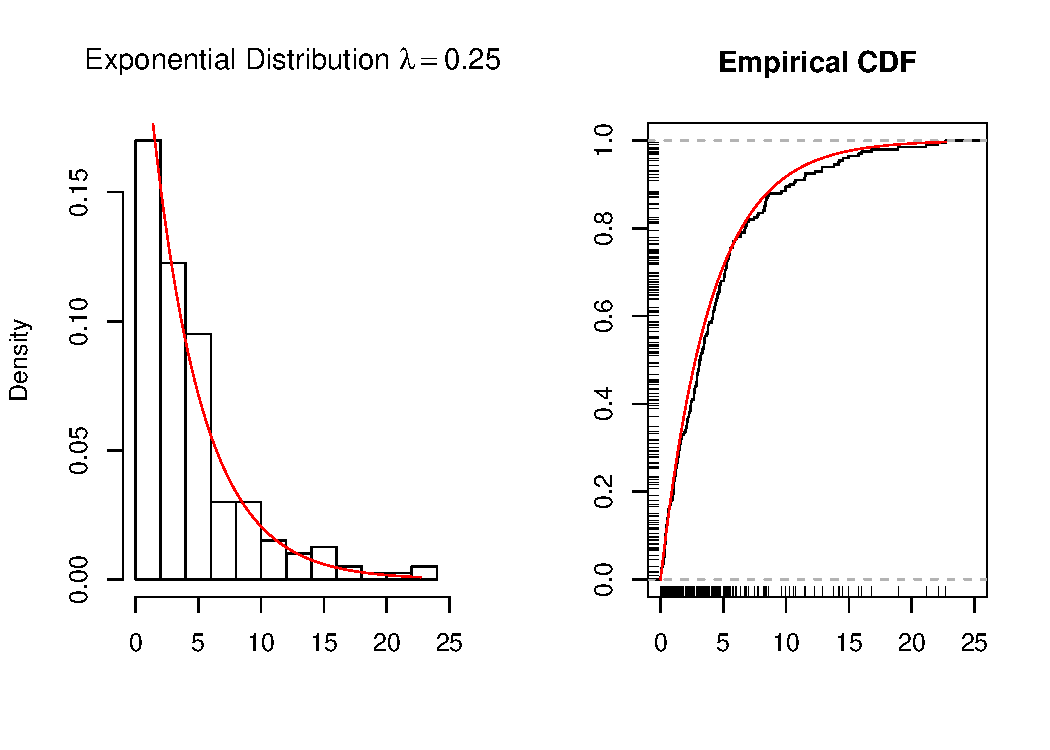
\includegraphics[width=4in]{RNG/images/expInvCDF.pdf}    
    \caption{The inverse CDF method was used to generate this sample of 200 from an exponential distribution with $\lambda = 0.25$.  Superimposed on the histogram (left) and empirical CDF (right) are the exponential density function and CDF, respectively.  The $y$-axis of the CDF plot shows a rug of the sample of  $200$ uniforms used to produce the exponentials, which appear as a rug on the $x$-axis of the same plot.}
    \label{fig:expInv}
  \end{center}
\end{figure}


We can compare moments of the sample with what we expect for a larger sample.
\begin{verbatim}
> y.e  = -4 *log(1- runif(10000))
> c(mean(y.e), var(y.e))
[1]  3.970798 15.611575
\end{verbatim}
In addition, we can generate a sample from R's built-in exponential
random-number generator and compare the moments.
\begin{verbatim}
> y.s = rexp(10000, .25)
> c(mean(y.s), var(y.s))
[1]  3.959364 15.889116
\end{verbatim}
These agree up to sampling error  (SE(mean)$ = 0.04$)
with the mean and SD of the distribution, $4$ and $16$ respectively.

Of course, this simulation does not prove that the inverse CDF method
gives us random values that follow the exponential distribution.  
We needed the math for that. 
However, the computer does allow us to explore the technique and
get an understanding of it for particular distributions.

We used the exponential distribution to illustrate the basics of the
inverse CDF method, but of course we had the built-in generator
available in R so there was no need.  Indeed, the generation
technique in R uses a different approach (given by Ahrens and Dieter).
One reason for avoiding the inverse CDF method is that computing
$F^{-1}(u)$ may be computationally expensive relative to another
approach.  However, the inverse CDF method is useful when the CDF is
invertible, that inverse function has a reasonably simple form, and
there are no built-in functions available to us.  For example, let's
consider a random variable whose distribution is given by the
triangular distribution.  This has a probability density given by

$$
  f(x) = 
  \begin{cases}%
   \frac{2(x - a)}{(b-a)(c-a)} & a \le x < c, \\
   \frac{2(b -x)}{(b-a)(b-c)} & c \le x \le b \\
   0 & x \not\in [a, b]    
  \end{cases}
$$
and is shown in Figure \ref{fig:triangularDensity}.
\begin{figure}[htbp]
  \begin{center}
    \leavevmode
    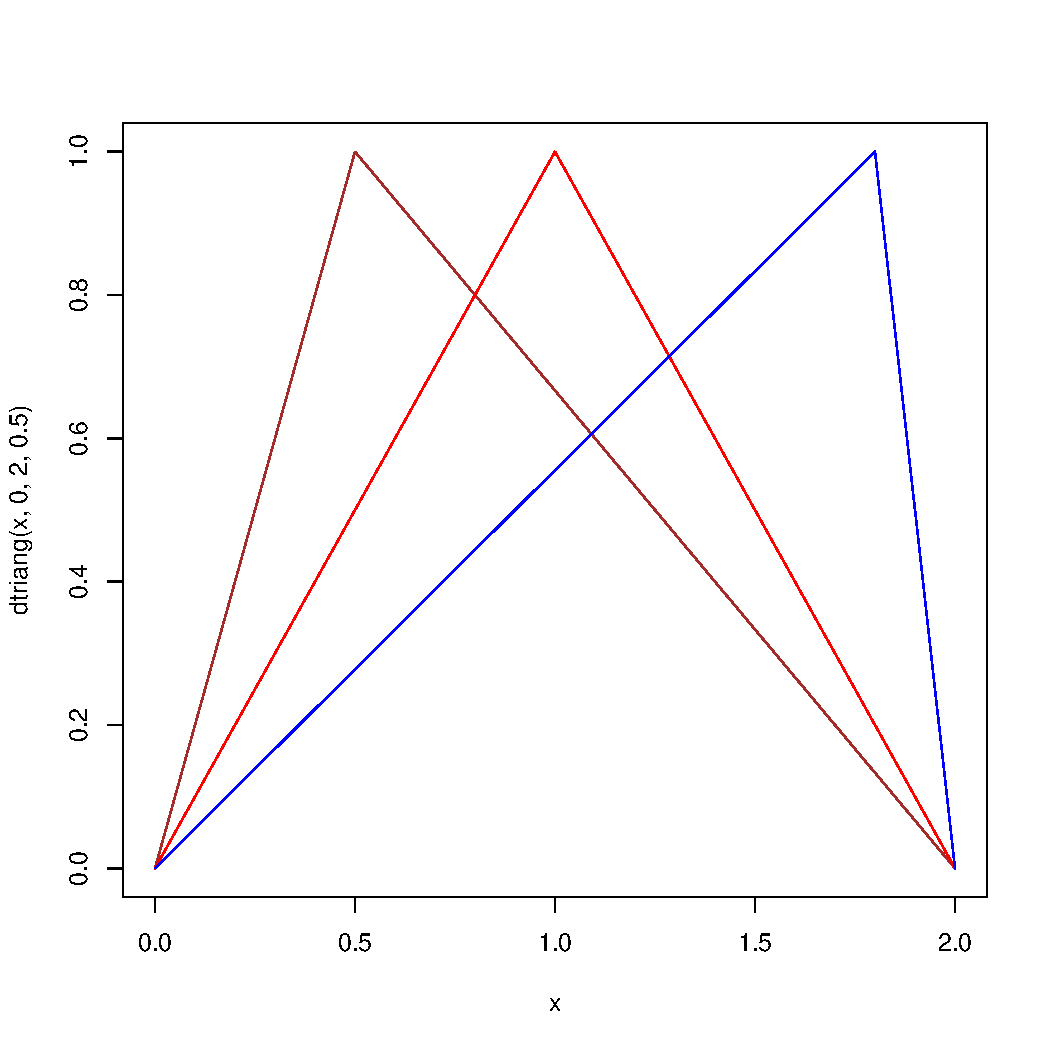
\includegraphics[width=4in]{RNG/images/triangularDensity.jpg}
    \caption{The probability density function of the triangular distribution.
   Shown here are three different triangular distributions
   on the  interval $[0, 2]$, with centers 
    $0.5$ (brown), $1$ (red), and $1.8$ (blue).
   }
    \label{fig:triangularDensity}
  \end{center}
\end{figure}
One can determine these formulae using
the simple facts that since this is a density, it 
must integrate to $1$, and that the 
area of a triangle is 
$1/2$ base $\times$ height.  We get
\begin{eqnarray*}
 1 & = & 1/2 (c-a)\times h + 1/2 (b-c) \times h \\
 h &=& 2/(b-a)
\end{eqnarray*}
Then, we have the two points on each line
and we can use the formula for a line.


We integrate the two components
in the density to get the CDF.
$$
  F(x) = 
  \begin{cases}
  \frac{(x - a)^2}{(b-a)(c-a)} & a \le x < c\\
                  1 - \frac{(b -x)^2}{(b-a)(b-c)} & c \le x \le b \\
                  0 & x < a \\
                  1 & x > b
  \end{cases}
$$

And finally, we must compute the inverse.  Unlike the case of the
exponential distribution, we have a quadratic function here and we
have two roots.
Taking the case where $c \le x < b$, we have
\begin{eqnarray*}
  Y = 1 - \frac{(b-x)^2}{(b-a)(b-c)} \\
  (1 - Y)(b-a)(b-c) = (b-x)^2 \\
  \sqrt{(1 - Y)(b-a)(b-c)} = b - x \\
\end{eqnarray*}
We can ignore the other root which is $-\sqrt{(1 - Y)(b-a)(b-c)}$
because $b - x$ must be positive as $x \le b$ and also $Y < 1$ since
it is our uniform random number.  We can similarly invert the other
term in the CDF.  All that is left is to determine the
intervals for which these two pieces in the inverse CDF apply.  The
splitting point on the X axis is $c$.  However, we need this on the
uniform - $[0,1]$ - scale.  The breakpoint on this scale is the
probability or area under the CDF up to the point $c$.
In other words, it is the area of the left triangle in 
the distribution. And this is
$1/2 (c-a) h$  = $(c-a)/(b-a)$. So the 
inverse of the CDF is 
$$
  F^{-1}(y) =
  \begin{cases}
    \sqrt{y(b-a)(c-a)} + a &  0 \le y < (c-a)/(b-a)\\
    b - \sqrt{(1 - y)(b-a)(b-c)} & (c-a)/(b-a) \le y \le 1 \\
    0 & y < 0 \\
    b & y > 1
  \end{cases}
$$

Now we can generate random numbers from a Triangular
distribution with parameters $(a, b, c)$ with $(a \le c \le b)$
using the R function
\begin{verbatim}
rtriang =
function(n, a = 0, b = 2, c = 1) {

  if(!(a <= c && c <= b)) 
   stop("Incorrect parameters")

  u = runif(n)
  ans = rep(0, length(u))
    
  base = b-a
  splitPoint = (c-a)/base
  leftside = (u < splitPoint)

  ans[leftside] = a + sqrt(u[leftside]*base*(c-a))
  ans[!leftside] = b - sqrt((1-u[!leftside])*base*(b-c)) 

  ans
}
\end{verbatim}

Now we can generate our samples and compare the result (Figure~\ref{fig:invTria})
% library(RNGTools)
\begin{verbatim}
x = rtriang(10000, 0, 3, 1)
hist(x, prob = TRUE, xlab= "X",
     main = "Triangular(0, 3, 1)")

points(density(x), type="l", col="blue")
curve(dtriang(x, 0, 3, 1), 0, 3, 
      add = TRUE, col = "red")
\end{verbatim}
Of course,  we get very good agreement with 
the only difference being sampling variability.

\begin{figure}[htbp]
  \begin{center}
    \leavevmode
    \includegraphics[width=4in]{RNG/images/TriaInvCDF.jpg}
    \caption{A histogram of a sample of 10,000 from the triangular distribution, with
    parameters $(0, 3, 1)$, i.e. endpoints are $0$ and $3$ and the peak is at $1$.
    Superimposed on the histogram is a density smooth of the sample (blue) and 
    the triangular pdf (red).}
    \label{fig:invTria}
  \end{center}
\end{figure}

In summary,
the inverse CDF approach works well if 
\begin{itemize}
\item we have a formula for the inverse CDF,
\item evaluating the formula for a given $u$ is not
excessively expensive,
\item and the software does not have a random number generator for
the desired distribution.
\end{itemize}


\section{Acceptance-Rejection}\label{sec:ars}
The acceptance-rejection method is an alternative to the inverse CDF method
when we cannot get the inverse, but we have a probability density function 
for the distribution.  Jon Von Neumann, the
``father of computer architecture'', devised a procedure that allows
us to create samples from essentially arbitrary density functions.  
The idea is quite simple and intuitive: 
\begin{itemize}
\item sample uniformly at random from a two-dimensional region 
 that encloses the probability density function (Figure~\ref{fig:ars}),
\item take (accept) only the points within our area of interest and ignore (reject)
those that fall outside this region, 
\item the $x$-coordinates of the accepted points form our 
sample, i.e. their probability distribution has density 
function $f$.
\end{itemize}

How this method works depends on two basic notions.  The first notion
relates probability to area. That is, consider points in
two-dimensions that are scattered randomly on a region, called
$\cal{A}$, in the plane.  This means that the probability of a point
falling in a sub-region ${\cal{B}} \subset {\cal{A}}$ is the same for all
subregions of the same area, and this chance is $Area
({\cal{B}})/Area({\cal{A}})$.

%The probability density function is a non-negative function where
%$$
%F(t) = \int_{-\infty}^t f(x) dx.
%$$
We apply this notion to a special region: the two-dimensional region
bounded by the $x$-axis and $y = f(x)$,
$$
{\cal{A}} = \{ (x,y) : 0 \le y \le f(x) \},
$$
And the subset that we look at is the region,
$$
{\cal{B}}_t = \{ (x,y) : 0 \le y \le f(x) ~\textrm{and } x \le t \}
$$
See Figure~\ref{fig:beta43} for an example.
If a point is sampled in two-dimensions at random from $\cal{A}$, then
the $x$-coordinate of the point follows the probabilty distribution with 
pdf $f$ and CDF $F$.  
To see why this is the case, we need only determine the CDF 
of the $x$-coordinate of the random-pair $(X, Y)$, 

\begin{eqnarray*}
Pr(X \le t) & = & Pr( (X, Y) \in {\cal{B}}_t ) \\ 
                & = & Area({\cal{B}}_t) / Area({\cal{A}}) \\
                & = & \int_{-\infty}^t f(x) dx\\
                & = & F(t)
\end{eqnarray*}             

We see from this derivation that if we could generate data from the
uniform distribution over $\cal{A}$, then we would have a random
sample from the probability distribution of interest.  Unfortunately,
it is typically the case that if we could generate samples uniformly
from $\cal{A}$ then we would also be able to generate samples via the
inverse CDF method.  The second basic property helps us out of this
bind.

The next notion is that when we take a random sample of $n$ points
from a larger region, say $\cal{C}$, and discard all of those
points which do not fall into $\cal{A}$, then the remaining points
form a uniform random sample in $\cal{A}$.  This means that if we want
a random sample of 100 points from $\cal{A}$, we generate a point from
$\cal{C}$, reject it if it is outside of $\cal{A}$, accept it if it is
inside $\cal{A}$, and continue in this way until $100$ points have
been accepted.  On average we would need to generate $100*Area
({\cal{C}})/Area({\cal{A}})$ points in order to yield $100$ points in
$\cal{A}$.  This means that if we have the tools to sample from
$\cal{C}$ then we simply discard those points that fall outside of the
region of interest $\cal{A}$, and take the $x$-coordinates of the
accepted points to get a sample from $F$.

Let's focus on a
particular density, say the $\beta(4, 3)$ shown in Figure
\ref{fig:beta43}.

\begin{figure}[htbp]
  \begin{center}
    \leavevmode
%   \includegraphics[width=3in]{RNG/images/beta43.jpg}
%\\
    \includegraphics[width=3in]{RNG/images/beta43Unif.jpg}
    \caption{Beta distribution - $\beta(4, 3)$}
    \label{fig:beta43}
  \end{center}
\end{figure}

Suppose we consider a rectangle that encloses this entire density,
namely the Cartesian region $[0,1] \times [0, c]$ for some $c$ as
shown in Figure \ref{fig:beta43Unif}.
Choosing our enveloping region as
close as possible to the region of interest  is highly desirable
because we will reject fewer observations. 
For our rectangular region, we want to chose $c$ to be the 
maximum of our density $f(x)$.  A little calculus allows us to find this.
Alternatively, we can use R to obtain an approximate answer
by evaluating the density at different points 
\begin{verbatim}
 max(dbeta(seq(0, 1, length = 100000), 4, 3)
\end{verbatim}
yielding $2.07$.

So, we need to generate random points in the region
 $[0, 1] \times [0,  2.07]$, and accept in our sample
those within the region under the density.  The question remains,
how can we do this practically and on a computer?

We break this
into two $1$ dimensional sampling steps. That is,
first we generate $X$ at random from the uniform distribution on 
$(0,1)$ and then we generate $U$ at random from the uniform
distribution on $(0, 2.07)$.  Together $(X, U)$ are uniformly
distributed over the desired region. 
\begin{verbatim}
 while(TRUE) {
   x = runif(1)
   u = runif(1, max = 2.07 * x)
   if(u < dbeta(x, 4, 3))
   break
}
\end{verbatim}

The proportion of samples that were accepted is $47.3\%$.
We see that the sample histogram is very close to the
density and the variation is just sampling error.
However, the larger region need not be rectangular in shape. 
In fact, a handy region to use 
is one where  we have a second probability density function, say $g()$, 
and a constant $c$ such that   $f(x) \le cg(x)$ for all $x$.
Then our larger region is ${\cal{A}} = \{  (x,y,): 0 \le y \le cg(x) \}$.
If we have a random number generator for $g$, it is easy to
generate points in $\cal{A}$:

\begin{enumerate}
\item Select $g()$ and $c$ such that  
    $c g(x) > f(x)$ for all $ x$.
\item Generate a random value, $X$,  from the distribution with density $g()$.
\item Generate a random value, $U$, from $U(0, c g(X))$.
\item Accept $X$ if $U \le f(X)$.
  Otherwise, return to step $2$.
\end{enumerate}

\begin{figure}[htbp]
  \begin{center}
    \leavevmode
    \includegraphics[width=4in]{RNG/images/ARSBetaUnif.jpg}
\\
    \includegraphics[width=4in]{RNG/images/ARSBetaTriangular.jpg}
    \caption{Acceptance/Rejection using the uniform distribution (top)
      and the triangular distribution (bottom)}
    \label{fig:betaUnif.jpg}
  \end{center}
\end{figure}

By choosing a better enveloping region, we can improve the acceptance
rate.  In the case of the $\beta(4,3)$ density, we can use a
triangular distribution as $g()$ and scale it to create an envelope
region. The particular choice of triangular distribution is $Tria(0, 1,
.8)$ and we choose $c$ to be $1.6$.  The plot in Figure
\ref{fig:betaUnif.jpg} shows this region.
\begin{verbatim}
acc = ars.eg(function(x) dbeta(x, 4,3), 
             function(x) dtria(x, 0, 1, .8), 
             1.6, 
             function(n) tria.inv(runif(n), 0, 1, .8), 
             10000)
\end{verbatim}
The acceptance rate for this is $62\%$.

\section{Example: Adhoc Networks}

Wireless networks are all around us.  Cell phones communicate with a
base-station to send and receive calls.  Calls are relayed from
base-station to base-station as the cell phone moves away from one and
closer to another.  A new idea of organizing networks is to avoid the
need for a central base-station that coordinates communications.
Instead, messages are relayed by ``hopping'' from one node to the next
to the next until it reaches its destination.  In other words, one can
send a message by using other devices in the network to relay the
message to the next device, and so on.  These are called \textit{ad
  hoc} networks because there is no centralized node or fixed
structure or topology for the network.  Devices can move over time,
and dynamically enter and exit the network, and so the route a message
takes from one device to another depends on the other nodes.

Ad hoc networks are very promising and becoming important.  At their
most immediately practical, ad hoc networks can allow nodes outside of
a regular network to communicate by piggy-backing off of nodes within
the network.  Think of driving along and being between base-stations
and so your cell phone call would be dropped, but, because of ad hoc
networks, your data is relayed through cell phones in other cars
closer to the base stations.  More ambitiously, ad hoc networks might
be used in controlling traffic on highways by allowing cars
closer to the base stations to communicate with each other.

A very basic aspect of ad hoc networks that researchers need to
understand is how the communication changes with respect to
broadcasting power.  If a set of nodes is connected, it means that it
is possible for any two nodes to communicate by having a message
travel along a path of nodes that are within broadcasting distance of
each other.  If the power level is very high then all nodes will be
able to broadcast directly to each other because increased power
levels allow one to send a message over a larger distance.  On the
other hand, if the power level is too low then a node may not be able
to connect to any other node, or the nodes may form two disjoint
connected subsets.  We are interested in studying the smallest power
level that leads to a connected network. We assume here that power
level is proportional to the radius, $R$, of a circle centered on the
node, and two nodes are in direct communication if the distance
between them is less than $R$.


 

\subsection{A probability model}

We would like to better understand how the smallest radius (such that
the network is connected) changes with different node configurations.
A probability model for messages moving on the network can help us
determine if the network is completely connected.

\begin{quote}
For a particular power level $R$, suppose a node has $k$
neighbors within $R$ of it.  Then a message located at this node will
hop at random to one of these $k$ nodes or will stay at its current
node, and these $k+1$ possible scenarios are equally likely.
\end{quote}

As such, the message hops around on the network in a random fashion,
and we can describe its random ``walk'' via a transition matrix for a
Markov Chain.  That is, for a message located at node $i$, $i = 1,
\ldots , N$ the chance it moves to node $j$, $j = 1, \ldots , N$, is
$0$ if these two nodes are further than $R$ away from each other, or
it is $1/k_i$ where $k_i$ is the number of nodes within $R$ of node
$i$.

For example, if $v_m$ is the $N \times 1$ vector of probabilities that
a message is at any one of the $N$ nodes at one ``instant'', then $P
v_m = v_{m+1}$ is the distribution of locations of the message at the
next instant, and $P v_{m+1} = v_{m+2}$ for the next instant, where
$P$ represents the matrix of transition probabilities, i.e. the
$i^{th}$ row of $P$ consists of $0$ for those nodes that are not
connected to node $i$ and $1/k_i$ for the $k_i$ nodes connected to
node $i$.  (We can also think of $v_m$ as the distribution of many
messages across the network.)

Mathematical properties of transition matrices tell us that the
distribution of the locations of the message settles down over time,
which implies that there is some $v$ where $P v = v$.  We see from
this equation that the steady state is the eigenvector of the
transition matrix associated with the eigenvalue of $1$.  Further, the
eigenvalues of $P$ are all real and less than or equal to one, and if
the network of nodes is fully connected, there is one unique
steady-state solution.  In this case, only the largest eigenvalue is
one, which implies that the size of the second largest eigenvalue is
key to determining if the network is connected.

\subsection{Generating nodes in the network}
To begin, we generate nodes in the hoc network.  Rather than
distributing nodes uniformly at random over the space, we model the
location of nodes by a density provided to us via the R function
\SFunction{nodeDensity}. A vector of $x$ and a vector of $y$
coordinates are taken as inputs to the function, and the return value
is a vector of values that are proportional to node density at the
$(x, y)$ pairs. This will be useful for sampling according to
the acceptance - rejection method.


% Place $75$ nodes at
%random on the $2$-dimensional grid shown in Figure~\ref{contourPlot},
%where the node density is proportional to the function shown in
%Figure~\ref{perspPlot}. Note the area of interest includes a ``river''
%where the density of nodes along the river is higher, except for
%locations in the river and along the banks of the river.  This density
%function is supplied as an

%%%%%%%%%%%%%%%%%

We create a picture of the region by generating values from a grid
using \SFunction{outer}, and plotting the results with
\SFunction{persp} and/or \SFunction{contour}, e.g.
\begin{verbatim}
x = 0:100
z = outer(x, x, nodeDensity)
persp(x, x, z, col = "lightblue", theta = 40, phi = 40,
         xlab = "0 to 100",  ylab = "0 to 100")
\end{verbatim}


The idea is that this is geographical region in which people live
and the density represents population density.  There are two
visible peaks that run along an arc of zero-density.  That arc is a
river in which nobody lives, but most people live along the river.
Fewer people live away from the river and there is another
region in the top right in which nobody lives.


\begin{figure}[htbp]
\begin{center}
\leavevmode
 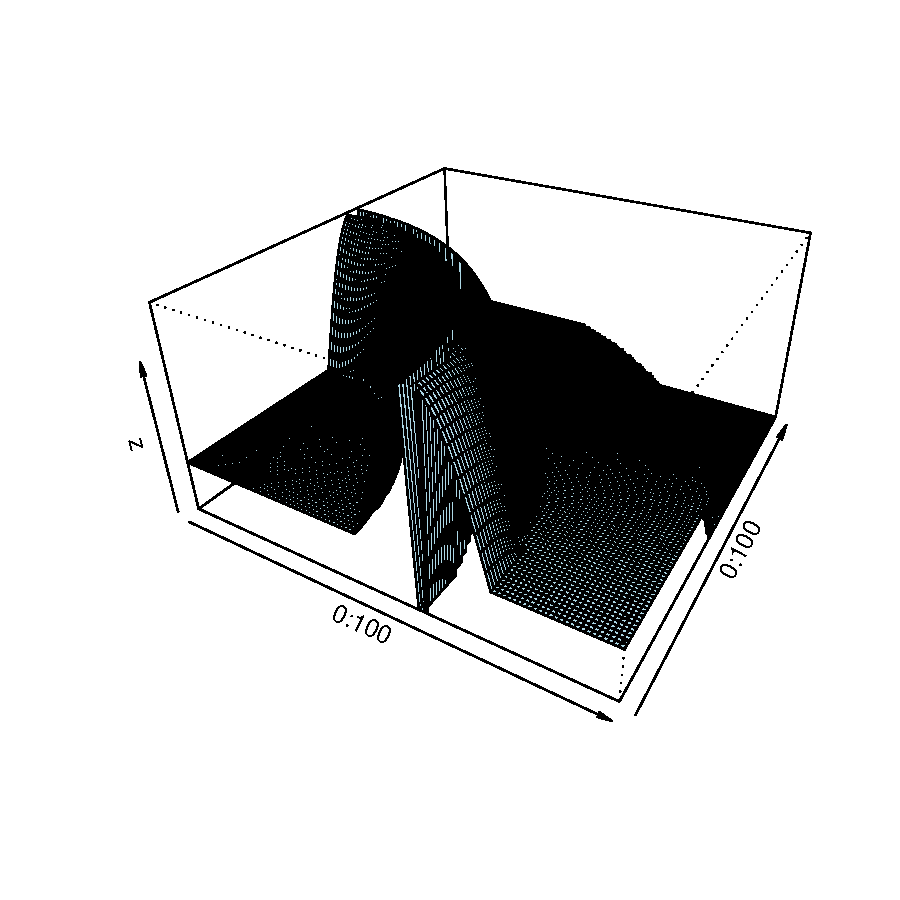
\includegraphics[width=4in]{RNG/images/perspRiver} % [width=6.5in]
\caption{A three-dimensional perspective plot of the region of interest.
Note that the river curves through the center of the region and no nodes
are located near the river.}
\label{perspPlot}
\end{center}
\end{figure}



This is a relatively straightforward application of
acceptance-rejection (AR) sampling.  It is hard to find a majorizing
density $g(x, y)$, so we use a simple 2-dimensional uniform.

We generate pairs $(x, y)$ from this 2-dimensional uniform by
generating $x$ and then $y$ from separate, independent uniform
distributions. In this case, both $X$ and $Y$ have the same
distribution, namely $U(0, 100)$.

For a given $(x, y)$ pair, we accept it if a random value from $U(0,
c')$ is less than $f(x, y)$, i.e. the density $f$ evaluated at the
potentially acceptable point.  All we need is to find the value of
$c'$ to complete the algorithm.  The value $c'$ satisfies $c' =
c\times g(x, y)$ for which $c' \ge f(x, y)$ for all $(x, y) \in
[0,100] \times [0, 100]$, i.e. that majorizes our density of interest.
Since $g(x, y)$, our 2-dimensional uniform, is constant, we are
concerned with its value, just the value for which $c' \ge f(x, y)$
for all $(x, y)$ pairs of interest.

To determine $c'$, we need to find the maximum value of $f(x, y)$.  We
cannot do this analytically without looking at the definition of $f(x,
y)$ in the \SFunction{nodeDensity} function. Even then, it may be hard
or impossible to solve exactly.  Instead, we can evaluate $f(x, y)$ at
many points on a grid of $(x, y)$ pairs and then look at the regions
at which the maxima occur.  For each of these potential maximum
points, we can break the neighborhood into grids of finer resolution
and continue to iteratively search for the maximum, getting
increasingly closer to the true answers.

Since we are only looking for a majorizing function rather than the
exact maximum, we can find the sample maximum and use a slightly
higher value.  Adding this ``fudge'' factor will just make our
acceptance/rejection mechanism slightly less efficient.

To find the maximum, we can use
\SFunction{outer} again.
{\footnotesize{
\begin{verbatim}
x = seq(0, 100)
z = outer(x, x, nodeDensity)
max(z)
\end{verbatim}
}}

The maximum is $ 3.983295$.
To zoom in on the neighborhoods,
we need to find out where the maxima occur.
\begin{verbatim}
r = x[row(z)[ z == max(z)]]
c = x[col(z)[ z == max(z)]]
\end{verbatim}
And these give us 
the pairs
$(61, 1)$ and $(1, 61)$.
Let's look at the region $[0, 2] \times [60, 62]$
\begin{verbatim}
x = seq(0, 2, length = 100)
y = seq(60, 62, length = 100)
z = outer(x, y, nodeDensity)
max(z)
\end{verbatim}
We get $3.983565$.  So we did find a slightly bigger value, but it is
likely that a value of $c' = 3.99$ will work well.

We can also take some protective measures in our code.  If we evaluate
$f(x, y)$ and find a value greater than $c'$, we will issue a
warning. Of course, it will be too late if we are already using random
values generated from this algorithm, but it is still a useful check
point.  We can even modify the algorithm to use the largest value of
$c'$ that it has encountered.


The following is a very simple and slow version of the
acceptance-rejection sampling approach for the problem.
{\footnotesize{
\begin{verbatim}
rDensity.slow = function(n = 100, c.prime = 3.99)  {
  if(n > 1)
    return(replicate(n, rDensity(1)))

  while(TRUE) {
     pos = runif(2, 0, 100)
     f = nodeDensity(pos[1], pos[2])
     if(runif(1, 0, c.prime) < f)
       return(pos)
   }
}
\end{verbatim}
}}
What this does is to accept a request for $n$ observations from the
density function \SFunction{nodeDensity}.  However, the function works
on just one observation at a time. So it calls itself $n$ times.  When
it is called with $n = 1$, it goes ahead and uses the AR approach.  It
continues indefinitely until it finds an acceptable point $(x, y)$.
It generates a target pair $(x, y)$ by sampling 2 observations from a
$U(0, 100)$, thus giving $x$ and $y$.  Then it evaluates $f(x, y)$ and
then compares this to a random observation from $U(0, c')$.  If it is
acceptable, the pair is returned; otherwise, it continues and
generates a new pair and checks that.


We can check that this does indeed give us $n$ pairs of $(x, y)$.
\begin{verbatim}
p = rDensity(10)
\end{verbatim}
We should check that they are all within the right range, i.e. $[0,
100]$.

How can we  determine whether the values come from that
density?
One approach is to take a large sample and count the number
in different bins.
\begin{verbatim}
p = rDensity(1000000)
x = seq(0, 100)
obs = table(cut(p[, 1], x), cut(p[,2], x))
\end{verbatim}
We can plot these counts as a function of 
X and Y.
\begin{verbatim}
x = seq(.5, length = 100)
persp(x, x, obs, theta = 30, phi = 30)
\end{verbatim}


\begin{figure}[htbp]
  \begin{center}
    \leavevmode
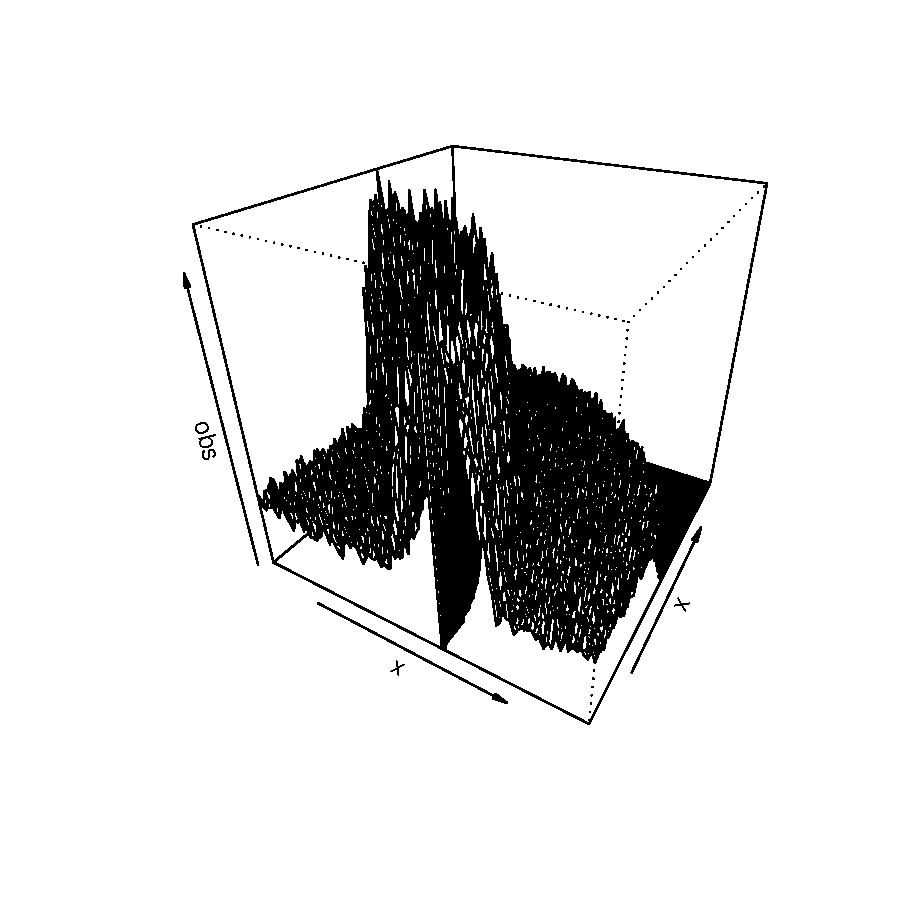
\includegraphics[width=4in]{RNG/images/nodeDensitySample.pdf}
    \caption{Samples from the acceptance-rejection method for the
      region in Figure~\ref{perspPlot}.}
    \label{fig:samplePerspPlot}
  \end{center}
\end{figure}
It is hard to see how good a fit this is.

\begin{comment}
Alternatively, we can draw the actual density
(as before) and then superimpose the scaled
counts:
{\footnotesize{
\begin{verbatim}
v = persp(x, x, outer(x, x, nodeDensity), phi = 30, theta = 30)
g = expand.grid(x, x)
oo = as.integer(obs)
points(trans3d(g[,1], g[,2], 4*oo/max(oo), v), col = "red", pch = "+")
\end{verbatim}
}}
%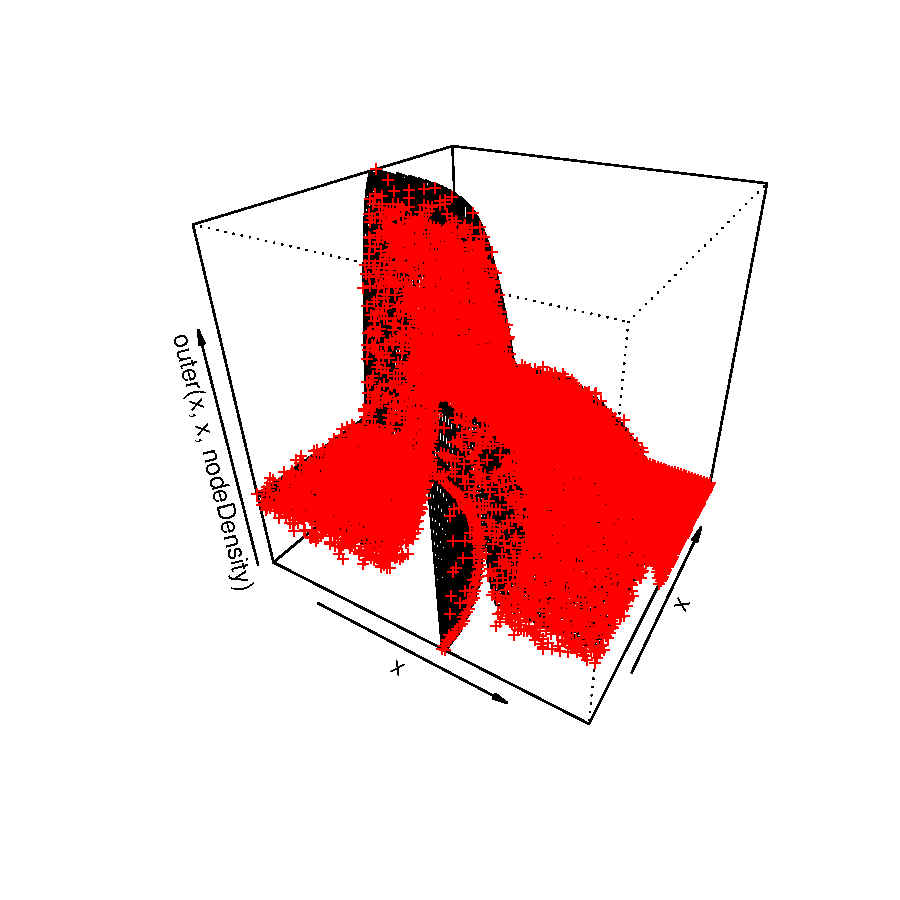
\includegraphics{RNG/images/nodeDensityPoints.pdf}
\end{comment}


We can compare the observed counts in each bin to the expected number
in each bin.  The expected number can be approximated by the average
$f(x, y)$ within the bin multiplied by the total number, i.e.
\Sexpression{nrow(p)}.
\begin{verbatim}
x = seq(.5, length = 100)
expected = outer(x, x, nodeDensity) * nrow(p)
\end{verbatim}
Of course, this approximation only works well when 
$f(x,y)$ is reasonably constant within a bin.
This is clearly not true for the high ridges.


We can also compute marginal and conditional distributions.  For $y =
0$, we should see the density being close to the front slice of the 2-D
density in the perspective plot:
\begin{verbatim}
curve(nodeDensity(x, rep(0, length(x))), 0, 100, 
      n = 10000)
points(seq(.5, length = 100), 
       as.numeric(4*obs[,1]/max(obs[, 1])), 
       col = "red")
\end{verbatim}
We can do this for arbitrary $y$
with the command
\begin{verbatim}
curve(nodeDensity(x, rep(y, length(x))), 0, 100, 
      n = 10000)
points(seq(.5, length = 100), 
      as.numeric(4*obs[,as.integer(y)]/max(obs[, 1])), 
      col = "red")
\end{verbatim}

\subsection{Improving the function}
Let's return to examining our function.  Note that we call
\SFunction{runif} for each pair $(x, y)$ and again for each $u$ to
determine if we accept the point.  The random number generation
functions in R can return $n$ values in a single call and this is much
more efficient than $n$ calls each returning a single observation.  We
can use this idea to make our function faster.  Firstly, we will try
to generate lots of values in a single step.  We will reject some, so
we will return and generate however many more are needed in the
subsequent attempts.  Each time, the number we need to generate should
be decreasing.  And in each iteration, we are generating numerous
values, not just a single value. So we are taking advantage of the
vectorized operations.

In addition to this speedup, we can also do a generic ``trick'' for
acceptance-rejection sampling.  Since we expect to reject some
proportion of the generated observations, we will generate more than
we need in the hope of getting the right number.  When asked for $n$
values, we generate $n' = k \times n$ values where $k > 1$.  By
carefully choosing $k$ (by theoretical or empirical reasoning), we can
find a trade-off between generating too many and not generating
enough.


A revised version of the function now looks like the following.  We
create an empty answer object which is a matrix with 2 columns and no
rows! We will add our acceptable observations as we generate them.  We
increase the number we will generate by multiplying by the
user-specifiable \SArg{factor}.  In our case, for every observation we
want, we will generate 3.  We then enter our acceptance-rejection
loop, continuing to sample until we have enough observations.  For
each iteration, we generate \Svariable{nmore} candidate points.  Then
we evaluate $f(x, y)$ at these points.  Then, we find out which are
acceptable by generating \Svariable{nmore} values from $U(0, c')$.
Note that we take advantage of the speed up here of generating many
values from this one distribution.  If we were not using a constant
majorizing density, we would not be able to do this. Instead, we would
have to generate each value from $U(0, c \times g(x, y))$.

Having determined the acceptable points, we append these to the answer
matrix. If the resulting matrix has $n$ or more rows, we can finish,
so we break from the loop.  Otherwise, we need to generate additional
observations and we need \Sexpression{n - row(ans)} of them.  So
again, we ask for \SArg{factor} times that many to take into account
the expected number of rejections.

At the end, we make certain to return only the first $n$ rows of the
answer matrix. If the caller asked for $n$, we must not give them back
$> n$ observations.

{\footnotesize{
\begin{verbatim}
rDensity =
function(n = 100, factor = 2.9, c.prime = 3.99)
{
   # Create an empty answer matrix with zero rows.
  ans = matrix(NA, 0, 2)

   # Determine how many we need to generate to get
   # the n that we want. 
  nmore = ceiling(factor*n)

   # This will store the proportion accepted at each iteration.
  rate <- numeric(0)
  
  while(TRUE) {
     pos = matrix(runif(2*nmore, 0, 100), ncol = 2)
     f = nodeDensity(pos[,1], pos[,2])
     
     acc = (runif(nmore, 0, c.prime) < f)
     ans <- rbind(ans, pos[acc,])

     rate[as.character(nmore)] <- sum(acc)/nmore
     
     if(nrow(ans) >= n)
        break

     nmore =  ceiling(factor * (n - nrow(ans)))
   }

   # Limit the result to just the first n rows
   # in case we ended up with more accepted.
   ans = ans[1:n,]

   # Put the rate information on the object
   attr(ans, "rate") <- rate
   ans
}
\end{verbatim}
}}



%%%%%%%%%%%%%%%%%

\subsection{Analysis of the adhoc network}
Search over different power levels and determine whether the nodes are
connected or not for the various power levels.  

Search over different power levels and determine whether the nodes are
connected or not for the various power levels.
Remember that for the set of nodes to be connected means that
it is possible for any two nodes to communicate by having a message
travel along nodes that are within broadcasting distance of each other.
If the power level is very high then all nodes will be able to broadcast
directly to each other. On the other hand, if the power level is too low
then a node may not be able to connect to any other node, or the nodes may
form two disjoint connected subsets.
We are interested in finding the smallest power level that leads to a
connected network. We assume here that power level is proportional
to the radius, $R$, of a circle centered on the node, and two nodes are
in direct communication if the distance between them is less than $R$.

How does the value of $R_c$, the smallest radius such that the
network is connected, change with different node configurations?
Repeat the above process of finding $R_c$ for 1000 random
node configurations generated according to the node density in
Figure~\ref{perspPlot}. Explore the distribution of $R_c$.
Is it symmetric, long tailed, similar to any of the ``standard''
distributions (normal, log-normal, exponential, gamma, etc.)
Plot the network of connected points for four of your 1000 node
configurations corresponding roughly to the min, median, mean,
and maximum values of $R_c$. 

Repeat the above process of finding $R_c$ for 1000 random
node configurations generated according to the node density in
Figure~\ref{perspPlot}. Explore the distribution of $R_c$.
Is it symmetric, long tailed, similar to any of the ``standard''
distributions (normal, log-normal, exponential, gamma, etc.)
Plot the network of connected points for four of your 1000 node
configurations corresponding roughly to the min, median, mean,
and maximum values of $R_c$. 

\begin{comment}
\begin{itemize}
\item \SFunction{.Random.seed} - used to set and save the seed for the
random number generator.
\item \SFunction{runif} - a pseudo-random number generator that takes vector
arguments.
\item \SFunction{eigen} - computes eigenvalues and eigenvectors. Be sure to
read about all of the arguments.
\item \SFunction{which} - can be very handy for figuring out which elements
in a vector have a certain property.
\item \SFunction{expand.grid} - a very useful function when searching over
a grid.
\item \SFunction{contour} - makes contour plots (used for the figures sown  
here). Be careful with the arguments, $z$ is a matrix corresponding to a
grid of $(x,y)$ values.
\item \SFunction{dist} - computes all pairwise distances between rows in a
matrix or data frame.
\end{itemize}
\end{comment}

 
\include{RNG/timingExampleShort}

\include{RNG/bootstrapSection}


\section{Markov Chain Monte Carlo - MCMC}
In most simulation contexts, we are interested in estimating the
expression $E_{f_X}[g(X)]$.
If we have i.i.d. samples from the random variable with density $f_X$
of the form $x_1, \ldots, x_n$, we can estimate this value
as
\begin{equation}\label{egx}
 E_{f_X}[g(X)] \approx \frac{1}{n} \sum_{i=1}^n g(x_i)
\end{equation}
The law of large numbers tells us that this is a good estimator.
Using different functions $g()$, we can obtain estimates for different
properties.  For example, $g(x) = x$ gives us the expectation of the
random variable.


Identical and independent values may be hard to sample from $f_X(x)$.
But we can use the estimator above in \ref{egx} if the $x_i$ are not
independent but sampled from $f_X(x)$ in proportion to $f_X()$.  The
computation of the variance is more complicated in these
circumstances, but the estimator is good.  This is because
\begin{equation}
  E_{f_X}[g(x)] = \int g(x) f_X(x) dx
\end{equation}
So if we can generate $x_i$ from $f_X()$ we can use Monte Carlo to
solve many problems.

The problem that we are now faced with is how to generate sample
values from the density $f_X(x)$, dependent or independent.  It turns
out that this is actually quite simple if we use what are called
Markov Chains.  Consider the following technique for generating a
sequence of random values.  Define $X_{t+1}$ by sampling from a
distribution that only depends on $X_t$, i.e. the current state of the
sequence.  In other words, we have a probability distribution given in
general terms as $P(X_{t+1} \vert X_t)$.  This sequence ${X_t}$ is
called a Markov chain.

To get the sequence started, we need a starting value $X_0$.  But
$X_{t}$ will depend on the value of $X_0$.  For many probability
distributions $P(X_{t+1} | X_t)$, it turns out that $P(. | X_0)$ is
independent of $X_0$ and it doesn't matter where we start.  And under
certain conditions, the sequence ${X_t}$ converges to a stationary
distribution, $\pi(x)$, which does not depend on $t$ or $X_0$.  Thus
for a sufficiently large value of $t$, $t_0$, $X_{t_{0} + 1}, X_{t_{0}
  + 2}, \ldots$ are samples (\textit{not} necessarily independent)
from the density $\pi(x)$.
So we can estimate $E_{g_X}[X]$ as 
\begin{equation}
  \frac{1}{n - t_0}\Sigma_{i = t_0}^n g(x_i)
\end{equation}


All that remains to use this technique is to create the Markov Chain.
In other words, we must specify the value $P(X_{t+1} \vert X_t)$ so
that we obtain the desired stationary distribution $f_X(x)$.  This
seems like a hard task, but it turns out to be quite simple.  Suppose
we have a distribution function $q(\cdot \vert X_t)$ which we will
call our \textit{proposal} distribution.  For a given $t$, we generate
a sample from a random variable $Y$ with this density.  We call $q()$
a proposal distribution because we don't use it directly to generate
$X_{t+1}$ in our sequence. Instead, we generate this new value but,
like acceptance/rejection sampling, we decide whether to accept it
under certain conditions.  Specifically, we use an decision algorithm
to accept or reject this new value.
The Hastings algorithm decides to accept this new value
with probability
$$
 min(1, \frac{f_X(Y)}{f_X(X_t)})
 $$ In other words, we toss a weighted coin with probability $ min(1,
 \frac{f_X(Y)}{f_X(X_t)})$ and if it turns up heads, we accept the new
 value $Y$ as the next step in the sequence, $X_{t+1}$.  If the coin
 ends up tails, we stay where we are and $X_{t+1} = X_t$.  This
 acceptance probability essentially favors $Y$ if $Y$ is more likely
 than the current value $X_{t}$.

The Metropolis-Hastings algorithm adds a variation to this.
Instead of looking at the likelihood ratio of $f_X(Y)/f_X(X_t)$,
it uses
$$
 \frac{q(X\vert Y) f_X(Y)}{q(Y\vert X) f_X(X)}
 $$ 
where $q$ is our proposal distribution again.
This yields nice properties that allow the Markov Chain to be
reversible and generally nicely behaved.

Regardless of which algorithm we use to accept or reject or our
proposal $Y$, the algorithm for generating the steps in the Markov
Chain are quite simple.

We need a function to generate a value from our proposal distribution.
This is the argument \SArg{r}.  To compute the acceptance probability,
we need $f_X()$, the stationary target density.  And if we are using
the Metropolis-Hastings algorithm we also need the density of the
proposal distribution given by \SArg{q}.  And we need a starting
point, $X_0$.  \SArg{n} says how many elements in the sequence we
should generate.  We need this to be large enough so that the chain
converges to $f_X()$ and yields sufficient sample values.
\begin{verbatim}
mcmc =
function(x.0 = 0, r, q, stationary, n = 1000, 
         algorithm = metropolis)
{
     xs = numeric(n+1)  # space for the answers
     xs[1] = x.0
     for(i in 1:n) {
       y = r(xs[i])   # Generate proposal
       k = algorithm(xs[i], y, stationary, q)
       xs[i+1] = ifelse(runif(1) <= k, y, xs[i])
       if(is.na(xs[i+1])) {
        stop("Problems in MCMC")
       }
     }

     class(xs) <- "mcmc"
     xs
}
\end{verbatim}


Let's generate a sample from a t-distribution with $10$ degrees of
freedom, $t(10)$.  This is the stationary distribution that is our
target.  We can use the R function \SFunction{dt} to compute the
density.  We will use a Normal distribution as our proposal
distribution with mean $X_t$ and variance $1$.  We can use
\SFunction{rnorm} to generate proposal values and \SFunction{dnorm} to
calculate the density in the Hastings algorithm.
We'll generate $10,000$ values and then look at the last
$5000$ to give this adequate time to ``burn in'' or converge
to $t(10)$. We'll chose a strange starting value of $-10$
to illustrate how this converges.
\begin{verbatim}
 xt = mcmc(-10, 
           r = function(x) rnorm(1, x), 
           q = function(x, y) dnorm(y, x), 
           stationary = function(x) dt(x, 10), 
           alg = hastings, 
           n = 10000)
\end{verbatim}
We can see how well the sample approximates the
true density $t(10)$ in Figure~\ref{fig:mcmcT10.jpg}

\begin{figure}[htbp]
  \begin{center}
    \leavevmode
    \includegraphics{RNG/images/mcmcT10.jpg}
    \caption{MCMC sample from $t(10)$.}
    \label{fig:mcmcT10.jpg}
  \end{center}
\end{figure}
This looks pretty close and within sampling variation.


The MCMC  approach to estimating $E[g(X)]$ and sampling dependent
values from a density is very powerful and is similar in ways to the
acceptance/rejection sampling we covered above.  One does have to
honor the conditions on the proposal and stationary distributions to
ensure that the Markov chain converges and converges to $f_X()$.


\section{Summary}
\begin{itemize}
\item 
\textit{Methods}: When random number generators do not exist for a particular probability
distribution, the inverse CDF method or the acceptance/rejection method
may be used. One is called the Inverse CDF method.
Another is Acceptance/Rejection sampling.  And a third is Markov Chain
Monte Carlo.

\item
\textit{Reproducabilty}: In order for others (and you) to reproduce your simulation results,
keep track of the initial value(s) used for the random number
generation, and report these value(s)
along with the specific random number generator used in your
simulation study.

\item
\textit{Monte Carlo}: Simulation studies offer useful comparisons of competing statistical
procedures, especially when the procedure is data-adaptive. For
example, if a \glossary{nuisance parameter},
must be specified for an estimator, we may want to compare
two techniques for selecting the parameter, where the techniques
depend on the data is a computationally complex way.  
Simulation studies, where we generate random numbers under various probability
distributions, help us study the behavior of statistical estimators.

\item
\textit{Resampling}: Resampling techniques, where we generate random samples from the observed data
itself rather than from a probability distribution, are very useful computational tools.
For example, they can approximate the sampling distribution of an estimator,
help us choose nuisance parameters for statistical procedures, and 
aid us in comparing the performance of various procedures.

\end{itemize}

\section{Exercises}

\begin{enumerate}

\item \textbf{Cross-validation}
Write an R function that provides the indices for $v$-fold cross-validation.

\begin{enumerate} 
\item \textbf{Inputs:} The parameters of the function include $n$ the
population size and $v$ the fold size.
Note both $n$ and $v$ are numeric vectors. The $v$ parameter must either be
the same length as $n$ or of length 1, in this case the same $v$ applies to
all elements in $n$.
The values for the fold size may range from 2 through $n$.
In addition, parameters are needed to determine how to handle
the case where $n$ is not an integer multiple of $v$ as explained
in the task paragraph below.

\item \textbf{Task:}
The main task is to divide the indices $1,2, \ldots ,n$
randomly into $v$ sugroups of equal size.  
If $v$ does not divide evenly into $n$ then a few possibilities are
to: fill the short subgroup with NAs, use a recycling rule to fill in
the short group, randomly fill in the short group.  You are encouraged
to find other approaches that make sense and include them as possibilities.

\item \textbf{Output:} The function returns a list, with one element
for each element in $n$.  These elements are data frames consisting
of the random indices arranged in $v$ columns. 
In the special case where $n$ is of length 1, then a single data frame
is returned.
\end{enumerate}


\item\label{prob:epa}
Consider the  Epanechnikov distribution, with probability
density function,
$$
\frac{3}{4}(1-u^2) ~ for~ -1<u<1
$$
and cumulative distribution function,
\begin{eqnarray*}
F(t) &=& 0 ~~~~~~~~~~~~~~~~~~~~~~ t < 0\\
 & = & \frac {1}{2} + \frac{3}{4} (t - \frac{t^3}{3}) ~~-1 < t  <1\\
  &=& 1 ~~~~~~~~~~~~~~~~~~~~~~~ t > 1
\end{eqnarray*}

\begin{enumerate}
\item Juxtapose plots of the pdf and the cdf of the Epanechnikov.

\item \textbf{Inverse CDF} Write a function to generate $n$ pseudo-random
values from the Epanechnikov  distribution.
Use the inverse CDF method to do this.  To find the inverse of the CDF use the
computer to evaluate $F$ at a dense sequence $t$ of values between -1 and 1
and do a reverse look-up of $t$ based on $p = F(t)$ .

\item \textbf{Monte Carlo}: Study the sampling distribution of  the mean and SD
of a sample 17 from the Epanechnikov distribution.  Use your function from the
step above to generate 2,000 samples of size 17 from the Epanechnikov distribution,
and make normal quantile plots of the 2,000 sample means and SDs.
Is it reasonable to assume that these statistics have a normal distribution?

\end{enumerate}

\item
 \textbf{Bootstrap} - Consider the sample data available at \\
\url{http://www.stat.berkeley.edu/users/statlabs/data/video.data}. \\
These data are from a simple random sample of 91 people in a population of 314.  A confidence interval for the mean is desired.  If the mean follows the
normal distribution (as with the average of 17 observations from the
Epanechnikov)  then a 95\% confidence interval would be
$( mean(x) - 2*SD(x), mean(x) + 2*SD(x))$.
But these data are highly skewed and it is not clear that the normal theory
holds in this case.
Instead, use the sample to form a bootstrap population of $314$,
and take 1,000 samples of size $91$ from the bootstrap population (with replacement).
 For each sample compute  the mean, and examine the distribution of these
 bootstrap means. Produce a 95\% confidence interval for the mean of
 the population using the bootstrap population.

\item  \textbf{Acceptance Rejection} Generating points  uniformly  under a curve can
be a bit tricky.  Consider these two approaches: generate points according to the 
uniform and accept only those that fall under the Epanechnikov pdf (see problem~\ref{prob:epa}).
Generate points uniform from -1 to 1 and for each point x, generate a y
uniformly from 0 to $f(x)$.  Do they both produce uniformly distributed
values under the Epanechnikov?  Why or why not?

\item
  Use the acceptance-rejection method to sample from a Gamma$(2, 3)$ density.  Write code for general shape and scale parameters, with scale $\ge 1$.  While one can do it generally, you can do experiments or write the code with a particular (non-trivial) $(\alpha, beta)$ pair.  But you should try it for different pairs then.

  One could use the uniform density to majorize the target distribution. Determine where the mode lies and what is the density at that value. That tells you what value of $c$ is needed to find $c g(x) \ge f(x), \forall x \in [0, \infty)$.

  To try to reduce the number of rejections, you can find a better majorizing function, $g(x)$.  You can try the double-exponential, defined as
$$
  g_X(x) = \frac{\theta}{2}e^{-\theta \vert x - \eta \vert}
$$ 
   choosing $\eta$ as the mode of $f_X(x)$.

   Use the computer to generate a sample from the Gamma$(2, 3)$ using these two majorizing densities. Ensure that the results are close to the Gamma$(2, 3)$ density by looking at Q-Q plots, or overlaying the Gamma density on a histogram of the sample values.

\item  Here are two approaches to sample from a double-exponential.
\begin{enumerate}
\item   Use the inverse CDF method.
\item   Work from exponential random number generator \SFunction{rexp} and randomly decide which values to make negative.
\item Determine which of these methods is more efficient. Is this efficiency a function of the parameter of the distribution?  Can one calculate the (expected) rejection rate mathematically?
\end{enumerate}

\item
Consider a Beta$(2, 3)$ random variable. It is defined for $x \in [0, 1]$.  Use the following two majorizing function to sample from the Bet$(2, 3)$ distribution via acceptance-rejection sampling.

\begin{enumerate}
\item Use the uniform majorizing function to sample from this density.
\item Use the Epanechnikov density defined in Problem~\ref{prob:epa}. If you scale and shift the range to $[0, 1]$, you end up with a Beta$(2, 2)$ density which has the ``special'' form
$$
  g_X(x) = 6x(1-x), \qquad x \in [0, 1]$$
\end{enumerate}
For each appraoch, find a value of $c$ such that $c g_X(x) \ge f_X(x)$
for all $x$ where $f_X(x)$ is the density of the Beta$(2, 3)$.  Use R
to get an approximate value for $c$, by plotting the curves and/or
evaluating the functions at many different values along the unit
interval.  Having decided on a value for $c$ for each majorizing
function, plot the sampling regions for the two majorizing functions,
i.e. $c g(x)$.  Can you tell which one will be have a higher
acceptance rate?


\item Note that when we asked for $n$ values in the updated
  \SFunction{rDensity} function, we got back 
a matrix as expected, but there was also an attribute
named \SArg{rate} attached to it which we can access
as 
\begin{verbatim}
z = rDensity(100)
attr(z, "rate")
\end{verbatim}
This is a named vector.  Each element tells us what proportion of the
generate candidate points were accepted.  The name for that element
tells us how many candidate points there were.  This information tells
us the empirical probability of acceptance.  Use this to calibrate the
function.  That is, these values are essentially estimates of $p$, the
probability of acceptance.  The variance of the estimate is $ \hat{p}
(1 - \hat{p})/n_i$, where $n_i$ is the number of items being sampled
of which $\hat{p}$ are rejected.  So we would want to take a weighted
average of these by using 1 over the variance as the weight.  And the
variance is essentially then 1 over the number of items that were up
for acceptance or rejection since $p$ is assumed to be the same.  So
the weights are
\begin{verbatim}
w = as.integer(names(attr(z, "rate")))
w = w/sum(w)
\end{verbatim}
and our estimate is 
\begin{verbatim}
sum(attr(z, "rate")* w)
\end{verbatim}

Update the function so that it can take a \SArg{factor} argument to
improve the efficiency of the sampling process.

\item 
Write a specialize plotting function that adds ``rug'' to the
  quantile-quantile plot of mixture problem. The ``yarns'' in the rug
  should be color-coded according to which distribution it was sampled
  from.  The resulting figure will look something like the following figure.

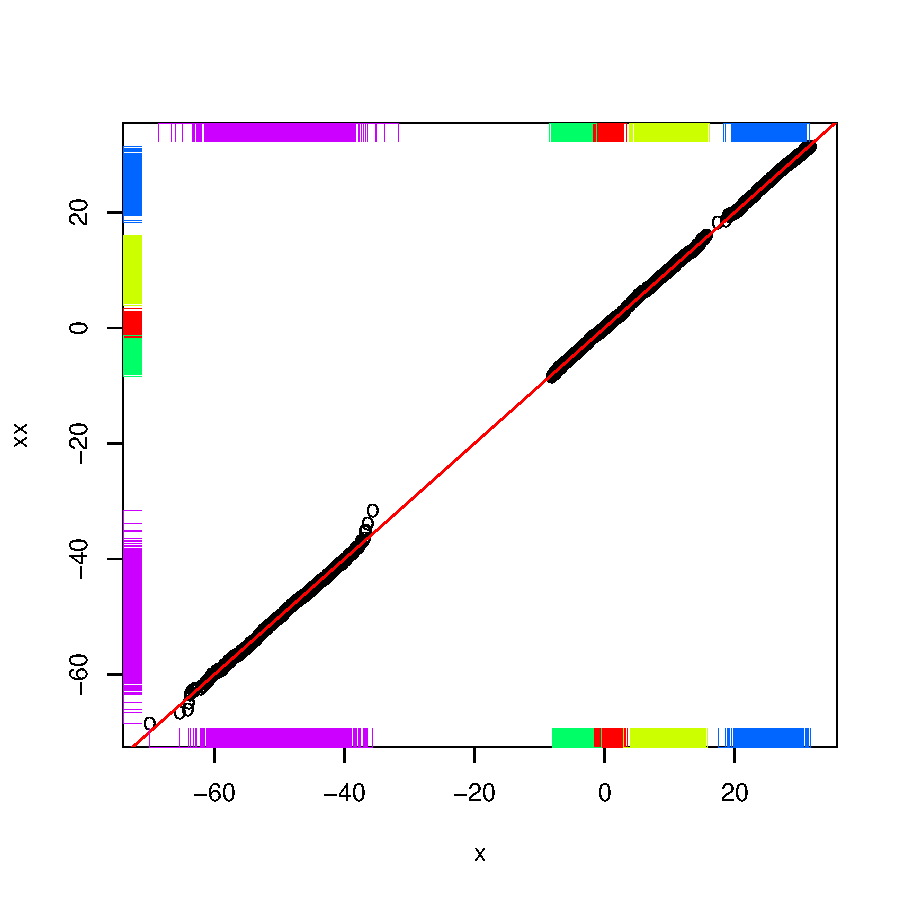
\includegraphics{RNG/images/QQEqualCount.pdf}   


\end{enumerate}

